\section{Dynamica}
\subsection{Opgave 1}
\subsubsection{Impuls}
De snelheid van het punt D en van het punt C die nodig is om de ogenblikkelijke impulsvector van het landingsgestel en het wiel te berekenen, werd al berekend in respectievelijk \eqref{eq:kin4.6} en \eqref{eq:kin2.8}.
\begin{itemize}
\item \textbf{Landingsgestel} 
\begin{equation}
\vec{p}_{l}^{'}=m_{l}\vec{v}_{d}^{'}=
\left[ \begin {array}{c} m_{l}\frac{1}{4}\,\omega_{i}\,l_{3}\\ \noalign{\medskip}m_{l}(v_{v}+\omega_{g}\, \left( l_{1}+\frac{3}{4}\,l_{4}) \right) \\ \noalign{\medskip}-m_{l}\frac{3}{4}\,\omega_{i}\,l_{4}\end {array} \right]
\label{eq:dyn1.1}
\end{equation}
\item \textbf{Wiel}
\begin{equation}
\vec{p}_{w}^{'}=m_{w}\vec{v}_{c}^{'}=
\left[ \begin {array}{c} m_{w}\omega_{i}\, \left( \sin \left( \beta
 \right) l_{4}-\cos \left( \beta \right) l_{3} \right) \\ \noalign{\medskip}m_{w}(-\cos \left( \beta \right) l_{4}\,\omega_{g}-\sin \left( \beta \right) l_{3}\,\omega_{g}+l_{1}\,\omega_{g}+v_{v})\\\noalign{\medskip}m_{w}\omega_{i}\, \left( \cos \left( \beta \right) l_{4}+\sin \left( \beta \right) l_{3} \right) \end {array} \right]
\label{eq:dyn1.2}
\end{equation}
\end{itemize}
\subsubsection{Verandering van impuls}
Ook de versnelling van de punten D en C zijn hier nodig en werden eerder al berekend in \eqref{eq:kin4.12} en \eqref{eq:kin2.15}.
\begin{itemize}
\item \textbf{Landingsgestel}
\begin{equation}
\frac{\mathrm{d}\vec{p}_{l}^{'}}{\mathrm{d}t}=m_{l}\vec{a}_{d}^{'}
=\left[ \begin {array}{c} m_{l}(-{\omega_{g}}^{2} \left( l_{1}+\frac{3}{4}\,l_{4} \right) +\frac{1}{4} \,\alpha_{i}\,l_{3}-\frac{3}{4}\,{\omega_{i}}^{2}l_{4})\\ \noalign{\medskip}m_{l}(a_{v}+\alpha_{g}\, \left( l_{1}+\frac{3}{4}\,l_{4} \right) +\frac{3}{4}\,\omega_{g}\,\omega_{i}\,l_{3})\\ \noalign{\medskip}m_{l}(-\frac{3}{4}\,\alpha_{i}\,l_{4}-\frac{1}{4}\,{\omega_{i}}^{2}l_{3})\end {array} \right]
\label{eq:dyn1.3}
\end{equation}
\item \textbf{Wiel}
\def\arraystretch{0.5}
\begin{equation}
\frac{\mathrm{d}\vec{p}_{w}^{'}}{\mathrm{d}t}=m_{w}\vec{a}_{c}^{'}
=\left[\begin{smallmatrix}m_{w}(-{\omega_{g}}^{2}\left(l_{1}-\cos\left(\beta\right)l_{4}-\sin\left(\beta\right)l_{3}\right)+\alpha_{i}\, \left(\sin\left(\beta\right)l_{4}-\cos\left(\beta\right)l_{3}\right)-{\omega_{i}}^{2}\left(-\cos\left(\beta\right)l_{4}-\sin \left(\beta\right)l_{3}\right))\\ \noalign{\medskip}m_{w}(a_{v}+\alpha_{g}\, \left( l_{1}-\cos \left( \beta \right) l_{4}-\sin \left(\beta\right)l_{3}\right)+3\,\omega_{g}\,\omega_{i}\,\left(\sin\left(\beta\right)l_{4}-\cos\left(\beta\right)l_{3}\right))\\ \noalign{\medskip}m_{w}(-\alpha_{i}\,\left(-\cos\left(\beta\right)l_{4}-\sin\left(\beta\right)l_{3}\right)-{\omega_{i}}^{2}\left(\sin \left(\beta\right)l_{4}-\cos\left(\beta\right)l_{3}\right))\end{smallmatrix}\right]
\label{eq:dyn1.4}
\end{equation}
\end{itemize}
\newpage
\subsection{Opgave 2}
\subsubsection{Impulsmoment}
\begin{itemize}
\item \textbf{Landingsgestel}

Zowel punt C als punt D zitten vast aan het landingsgestel en hebben dus bijgevolg dezelfde hoeksnelheid. Voor $\vec{\omega}_{c}$ zie \eqref{eq:kin1.2}.

Om de inertiematrix van het landingsgestel te kunnen gebruiken in onze formule dienen we ze eerst om te zetten naar het $x'y'z'$-assenstelsel.
\begin{equation}
\begin{split}
I_{l}^{'}&=R^{x'''y'''z''' \rightarrow x'y'z'}I_{l}^{'''}\\
&=\begin{bmatrix}
\cos(\beta)	&			0			&\sin(\beta)\\
0						&			1			&			0		 \\
-\sin(\beta)&			0			&\cos(\beta)\\
\end{bmatrix}
\begin{bmatrix}
I_{l,x'''x'''}&0&0\\
0&I_{l,y'''y'''}&0\\
0&0&I_{l,z'''z'''}\\
\end{bmatrix}\\
&=\begin{bmatrix}
\cos(\beta)I_{l,x'''x'''}	&			0			&\sin(\beta)I_{l,z'''z'''}\\
0						&			I_{l,y'''y'''}			&			0		 \\
-\sin(\beta)I_{l,x'''x'''}&			0			&\cos(\beta)I_{l,z'''z'''}\\
\end{bmatrix}
\end{split}
\label{eq:dyn2.1}
\end{equation}
\begin{equation}
\begin{split}
\vec{L}_{l}^{'}&=I_{l}^{'}\vec{\omega}_{d}^{'}=I_{l}^{'}\vec{\omega}_{c}^{'}\\
&=\begin{bmatrix}
\cos(\beta)I_{l,x'''x'''}	&			0			&\sin(\beta)I_{l,z'''z'''}\\
0						&			I_{l,y'''y'''}			&			0		 \\
-\sin(\beta)I_{l,x'''x'''}&			0			&\cos(\beta)I_{l,z'''z'''}\\
\end{bmatrix}
\begin{bmatrix}
-\omega_{w}\cos(\beta)	\\
\omega_{i}						\\
\omega_{g}+\omega_{w}\sin(\beta)	\\
\end{bmatrix}\\
&=\begin{bmatrix}
-\cos^{2}(\beta)I_{l,x'''x'''}\omega_{w}+\sin(\beta)I_{l,z'''z'''}(\omega_{g}+\omega_{w} \sin(\beta))	\\
I_{l,y'''y'''}\omega_{i}						\\
\sin(\beta)\cos(\beta)I_{l,x'''x'''}\omega_{w}+\cos(\beta)I_{l,z'''z'''}(\omega_{g}+\omega_{w} \sin(\beta))	\\
\end{bmatrix}
\end{split}
\label{eq:dyn2.2}
\end{equation}
\item \textbf{Wiel}

Het impulsmoment van het wiel wordt bijna op exact dezelfde wijze berekend.
\begin{equation}
\begin{split}
I_{w}^{'}&=R^{x''''y''''z'''' \rightarrow x'y'z'}I_{w}^{''''}\\
&=\begin{bmatrix}
\cos(\beta)	&			0			&\sin(\beta)\\
0						&			1			&			0		 \\
-\sin(\beta)&			0			&\cos(\beta)\\
\end{bmatrix}
\begin{bmatrix}
I_{w,x''''x''''}&0&0\\
0&I_{w,y''''y''''}&0\\
0&0&I_{w,z''''z''''}\\
\end{bmatrix}\\
&=\begin{bmatrix}
\cos(\beta)I_{w,x''''x''''}	&		0		&\sin(\beta)I_{w,z''''z''''}\\
0			&			I_{w,y''''y''''}			&		0		 \\
-\sin(\beta)I_{w,x''''x''''}&		0		&\cos(\beta)I_{w,z''''z''''}\\
\end{bmatrix}
\end{split}
\label{eq:dyn2.3}
\end{equation}
\begin{equation}
\begin{split}
\vec{L}_{w}^{'}&=I_{w}^{'}\vec{\omega}_{c}^{'}\\
&=\begin{bmatrix}
\cos(\beta)I_{w,x''''x''''}	&		0		&\sin(\beta)I_{w,z''''z''''}\\
0			&			I_{w,y''''y''''}			&		0		 \\
-\sin(\beta)I_{w,x''''x''''}&		0		&\cos(\beta)I_{w,z''''z''''}\\
\end{bmatrix}
\begin{bmatrix}
-\omega_{w}\cos(\beta)	\\
\omega_{i}						\\
\omega_{g}+\omega_{w}\sin(\beta)	\\
\end{bmatrix}\\
&=\begin{bmatrix}
-\cos^{2}(\beta)I_{w,x''''x''''}\omega_{w}+\sin(\beta)I_{w,z''''z''''}(\omega_{g}+\omega_{w} \sin(\beta))	\\
I_{w,y''''y''''}\omega_{i}						\\
\sin(\beta)\cos(\beta)I_{w,x''''x''''}\omega_{w}+\cos(\beta)I_{w,z''''z''''}(\omega_{g}+\omega_{w} \sin(\beta))	\\
\end{bmatrix}
\end{split}
\label{eq:dyn2.4}
\end{equation}
\end{itemize}
\newpage
\subsubsection{Verandering van impulsmoment}
\begin{itemize}
\item \textbf{Landingsgestel}

Om de verandering van impulsmomentvector te kunnen berekenen, werken we eerst de relatieve component uit.
\begin{equation}
\begin{split}
\left(\frac{\mathrm{d}\vec{L}_{l}^{'}}{\mathrm{d}t}\right)_{rel} &= I_{l}^{'}\vec{\alpha}_{d}^{'}=I_{l}^{'}\vec{\alpha}_{c}^{'}\\
&=\begin{bmatrix}
\cos(\beta)I_{l,x'''x'''}	&			0			&\sin(\beta)I_{l,z'''z'''}\\
0						&			I_{l,y'''y'''}			&			0		 \\
-\sin(\beta)I_{l,x'''x'''}&			0			&\cos(\beta)I_{l,z'''z'''}\\
\end{bmatrix}
\begin{bmatrix}
\alpha_{w}\cos(\beta)-\omega_{i}\omega_{g}+\omega_{i}\omega_{w}\sin{\beta}\\
\alpha_{i}-\omega_{g}\omega_{w}\cos{\beta}\\
\alpha_{g}-	\alpha_{w} \sin(\beta)+\omega_{i}\omega_{w}\cos{\beta}\\
\end{bmatrix}\\
&=\left[\begin{smallmatrix}
\cos(\beta)I_{l,x'''x'''}(\alpha_{w}\cos(\beta)-\omega_{i}\omega_{g}+\omega_{i}\omega_{w}\sin{\beta})+\sin(\beta)I_{l,z'''z'''}(\alpha_{g}-	\alpha_{w} \sin(\beta)+\omega_{i}\omega_{w}\cos{\beta})\\
I_{l,y'''y'''}(\alpha_{i}-\omega_{g}\omega_{w}\cos{\beta})\\
-\sin(\beta)I_{l,x'''x'''}(\alpha_{w}\cos(\beta)-\omega_{i}\omega_{g}+\omega_{i}\omega_{w}\sin{\beta})+\cos(\beta)I_{l,z'''z'''}(\alpha_{g}-	\alpha_{w} \sin(\beta)+\omega_{i}\omega_{w}\cos{\beta})\\
\end{smallmatrix}\right]\\
\end{split}
\label{eq:dyn2.5}
\end{equation}
De volledige vergelijking \footnote{Hier worden $I_{l,x'''x'''}$, $I_{l,y'''y'''}$ en $I_{l,z'''z'''}$ afgekort als respectievelijk $I_{l,x'''}$, $I_{l,y'''}$ en $I_{l,z'''}$ om de omvang van de matrix te beperken.} voor de verandering van het impulsmoment gaat als volgt (met $\vec{\Omega}_{c}$ gelijk aan $\vec{\omega}_{c}$).
\begin{equation*}
\begin{split}
\frac{\mathrm{d}\vec{L}_{l}^{'}}{\mathrm{d}t}&=\left(\frac{\mathrm{d}\vec{L}_{l}^{'}}{\mathrm{d}t}\right)_{rel} + \vec{\Omega}_{c}^{'} \times \vec{L}_{l}^{'}\\
&=\left[\begin{smallmatrix}
\cos(\beta)I_{l,x'''x'''}(\alpha_{w}\cos(\beta)-\omega_{i}\omega_{g}+\omega_{i}\omega_{w}\sin{\beta})+\sin(\beta)I_{l,z'''z'''}(\alpha_{g}-	\alpha_{w} \sin(\beta)+\omega_{i}\omega_{w}\cos{\beta})\\
I_{l,y'''}(\alpha_{i}-\omega_{g}\omega_{w}\cos{\beta})\\
-\sin(\beta)I_{l,x'''}(\alpha_{w}\cos(\beta)-\omega_{i}\omega_{g}+\omega_{i}\omega_{w}\sin{\beta})+\cos(\beta)I_{l,z'''}(\alpha_{g}-	\alpha_{w} \sin(\beta)+\omega_{i}\omega_{w}\cos{\beta})\\
\end{smallmatrix}\right]\\
\end{split}
\end{equation*}
\begin{equation}
+\left|\begin{smallmatrix}
e_{x}&e_{y}&e_{z}\\
-\omega_{w}\cos(\beta)&\omega_{i}&\omega_{g}+\omega_{w}\sin(\beta)\\-\cos^{2}(\beta)I_{l,x'''}\omega_{w}+\sin(\beta)I_{l,z'''}(\omega_{g}+\omega_{w} \sin(\beta))&I_{l,y'''}\omega_{i}&\sin(\beta)\cos(\beta)I_{l,x'''}\omega_{w}+\cos(\beta)I_{l,z'''}(\omega_{g}+\omega_{w} \sin(\beta))\\
\end{smallmatrix}\right|
\label{eq:dyn2.6}
\end{equation}
%&=\begin{bmatrix}
%\cos(\beta)I_{l,x'''x'''}(\alpha_{w}\cos(\beta)-\omega_{i}\omega_{g}+\omega_{i}\omega_{w}\sin{\beta})+\sin(\beta)I_{l,z'''z'''}(\alpha_{g}-	\alpha_{w} \sin(\beta)+\omega_{i}\omega_{w}\cos{\beta})
%\omega_{i}(\sin(\beta)\cos(\beta)I_{l,x'''x'''}\omega_{w}+\cos(\beta)I_{l,z'''z'''}(\omega_{g}+\omega_{w} \sin(\beta)))-(\omega_{g}+\omega_{w} \sin(\beta)I_{l,y'''y'''}\omega_{i}\\
%I_{l,y'''y'''}(\alpha_{i}-\omega_{g}\omega_{w}\cos{\beta})+\omega_{w}\cos(\beta)(\sin(\beta)\cos(\beta)I_{l,x'''x'''}\omega_{w}+\cos(\beta)I_{l,z'''z'''}(\omega_{g}+\omega_{w} \sin(\beta)))+(\omega_{g}+\omega_{w} \sin(\beta))(-\cos^{2}(\beta)I_{l,x'''x'''}\omega_{w}+\sin(\beta)I_{l,z'''z'''}(\omega_{g}+\omega_{w} \sin(\beta)))\\
%-\sin(\beta)I_{l,x'''x'''}(\alpha_{w}\cos(\beta)-\omega_{i}\omega_{g}+\omega_{i}\omega_{w}\sin{\beta})+\cos(\beta)I_{l,z'''z'''}(\alpha_{g}-	\alpha_{w} \sin(\beta)+\omega_{i}\omega_{w}\cos{\beta})-\cos(\beta)\omega_{w}\omega_{i}I_{l,y'''y'''}-\omega_{i}(-\cos^{2}(\beta)I_{l,x'''x'''}\omega_{w}+\sin(\beta)I_{l,z'''z'''}(\omega_{g}+\omega_{w} \sin(\beta))&I_{l,y'''y'''}\omega_{i}&\sin(\beta)\cos(\beta)I_{l,x'''x'''}\omega_{w}+\cos(\beta)I_{l,z'''z'''}(\omega_{g}+\omega_{w} \sin(\beta)))\\
%\end{bmatrix}
De vergelijking wordt niet verder uitgewerkt omdat dat ons te ver zou drijven in het louter uitrekenen van determinanten. Het uiteindelijke resultaat is uitgedrukt in het $x'y'z'$-assenstelsel en moet nog vermenigvuldigd worden met een transformatiematrix om ze naar het wereldassenstelsel om te zetten.
\begin{equation}
\frac{\mathrm{d}\vec{L}_{l}}{\mathrm{d}t}=R^{x'y'z' \rightarrow xyz}\frac{\mathrm{d}\vec{L}_{l}^{'}}{\mathrm{d}t}
\label{eq:dyn2.7}
\end{equation}
\item \textbf{Wiel}

De verandering van het impulsmoment van het wiel wordt bijna op exact dezelfde wijze berekend.
\begin{equation}
\begin{split}
\left(\frac{\mathrm{d}\vec{L}_{w}^{'}}{\mathrm{d}t}\right)_{rel} &= I_{w}^{'}\vec{\alpha}_{c}^{'}\\
&=\begin{bmatrix}
\cos(\beta)I_{w,x'''x'''}	&			0			&\sin(\beta)I_{w,z'''z'''}\\
0						&			I_{w,y'''y'''}			&			0		 \\
-\sin(\beta)I_{w,x'''x'''}&			0			&\cos(\beta)I_{w,z'''z'''}\\
\end{bmatrix}
\begin{bmatrix}
\alpha_{w}\cos(\beta)-\omega_{i}\omega_{g}+\omega_{i}\omega_{w}\sin{\beta}\\
\alpha_{i}-\omega_{g}\omega_{w}\cos{\beta}\\
\alpha_{g}-	\alpha_{w} \sin(\beta)+\omega_{i}\omega_{w}\cos{\beta}\\
\end{bmatrix}\\
&=\left[\begin{smallmatrix}
\cos(\beta)I_{w,x'''x'''}(\alpha_{w}\cos(\beta)-\omega_{i}\omega_{g}+\omega_{i}\omega_{w}\sin{\beta})+\sin(\beta)I_{w,z'''z'''}(\alpha_{g}-	\alpha_{w} \sin(\beta)+\omega_{i}\omega_{w}\cos{\beta})\\
I_{w,y'''y'''}(\alpha_{i}-\omega_{g}\omega_{w}\cos{\beta})\\
-\sin(\beta)I_{w,x'''x'''}(\alpha_{w}\cos(\beta)-\omega_{i}\omega_{g}+\omega_{i}\omega_{w}\sin{\beta})+\cos(\beta)I_{w,z'''z'''}(\alpha_{g}-	\alpha_{w} \sin(\beta)+\omega_{i}\omega_{w}\cos{\beta})\\
\end{smallmatrix}\right]\\
\end{split}
\label{eq:dyn2.8}
\end{equation}
\begin{equation*}
\begin{split}
\frac{\mathrm{d}\vec{L}_{w}^{'}}{\mathrm{d}t}&=\left(\frac{\mathrm{d}\vec{L}_{w}^{'}}{\mathrm{d}t}\right)_{rel} + \vec{\Omega}_{c}^{'} \times \vec{L}_{w}^{'}\\
&=\left[\begin{smallmatrix}
\cos(\beta)I_{w,x'''x'''}(\alpha_{w}\cos(\beta)-\omega_{i}\omega_{g}+\omega_{i}\omega_{w}\sin{\beta})+\sin(\beta)I_{w,z'''z'''}(\alpha_{g}-	\alpha_{w} \sin(\beta)+\omega_{i}\omega_{w}\cos{\beta})\\
I_{w,y'''}(\alpha_{i}-\omega_{g}\omega_{w}\cos{\beta})\\
-\sin(\beta)I_{w,x'''}(\alpha_{w}\cos(\beta)-\omega_{i}\omega_{g}+\omega_{i}\omega_{w}\sin{\beta})+\cos(\beta)I_{w,z'''}(\alpha_{g}-	\alpha_{w} \sin(\beta)+\omega_{i}\omega_{w}\cos{\beta})\\
\end{smallmatrix}\right]
\end{split}
\end{equation*}
\begin{equation}
+\left|\begin{smallmatrix}
e_{x}&e_{y}&e_{z}\\
-\omega_{w}\cos(\beta)&\omega_{i}&\omega_{g}+\omega_{w}\sin(\beta)\\-\cos^{2}(\beta)I_{w,x'''}\omega_{w}+\sin(\beta)I_{w,z'''}(\omega_{g}+\omega_{w} \sin(\beta))&I_{w,y'''}\omega_{i}&\sin(\beta)\cos(\beta)I_{w,x'''}\omega_{w}+\cos(\beta)I_{w,z'''}(\omega_{g}+\omega_{w} \sin(\beta))\\
\end{smallmatrix}\right|
\label{eq:dyn2.9}
\end{equation}
\begin{equation}
\frac{\mathrm{d}\vec{L}_{w}}{\mathrm{d}t}=R^{x'y'z' \rightarrow xyz}\frac{\mathrm{d}\vec{L}_{w}^{'}}{\mathrm{d}t}
\label{eq:dyn2.10}
\end{equation}
\end{itemize}
\newpage
\subsection{Opgave 3}
\begin{figure}[H]
\center
  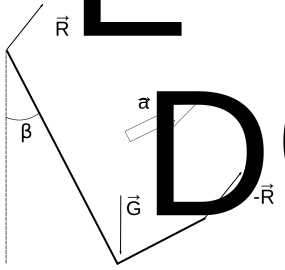
\includegraphics[width=0.45\linewidth]{./images/Vrijlichaamdiagram-1.png}
	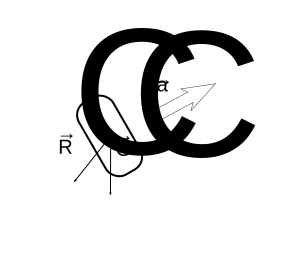
\includegraphics[width=0.45\linewidth]{./images/Vrijlichaamdiagram-2.png}
  \caption{Vrijlichaamsdiagramma van landingsgestel en wiel}
  \label{image:diagramma}
\end{figure}
Uit het vrijlichaamsdiagram van het landingsgestel volgt volgend krachtenevenwicht:
\begin{equation}
\begin{split}
-\vec{R}_{c}+\vec{G}_{d}+\vec{R}_{b} &= m_{l} \cdot \vec{a}_{d}\\
&=
\end{split}
\label{eq:dyn2.5}
\end{equation}
\subsection{Opgave 4}
\subsection{Opgave 5}